\documentclass[12pt,a4paper]{jbook}
\usepackage{mm-thesis}
\usepackage[dvipdfmx]{graphicx}
\usepackage{cite}
\usepackage{comment}
\usepackage{docmute}
\usepackage{color}
\usepackage{moreverb}
\usepackage{listings}
\usepackage{ascmac}
%\usepackage{amsmath}
%\usepackage{amsthm}
%\usepackage{amsfonts}

\lstset{
	%枠外での自動改行
 	breaklines = true,
 	%標準の書体
 	basicstyle = {\small},
 	%枠 "t"は上に線を記載, "T"は上に二重線を記載
	%他オプション:leftline,topline,bottomline,lines,single,shadowbox
 	frame = TB,
 	%タブの大きさ
 	tabsize = 2,
 	%キャプションの場所("tb"ならば上下両方に記載)
 	captionpos = t,
 	%行番号の位置
 	numbers = left,
 	%自動改行後のインデント量(デフォルトでは20[pt])	
 	breakindent = 30pt,
	%左右の位置調整 	
 	xleftmargin=30pt,
 	xrightmargin=30pt,
	%プログラム言語(複数の言語に対応,C,C++も可)
 	%language = Python, 	
 	%背景色と透過度
 	%backgroundcolor={\color[gray]{.90}},
 	%コメントの書体
 	%commentstyle = {\itshape \color[cmyk]{1,0.4,1,0}},
 	%関数名等の色の設定
 	%classoffset = 0,
 	%キーワード(int, ifなど)の書体
 	%keywordstyle = {\bfseries \color[cmyk]{0,1,0,0}},
 	%表示する文字の書体
 	%stringstyle = {\ttfamily \color[rgb]{0,0,1}},
 	%frameまでの間隔(行番号とプログラムの間)
 	%framesep = 5pt,
 	%行番号の間隔
 	%stepnumber = 1,
	%行番号の書体
 	%numberstyle = \tiny,
}
\renewcommand{\lstlistingname}{Code}
\begin{document}

\chapter{既存のウェブセキュリティモデル}
この章では、セキュリティモデルの説明と、本研究の提案モデルの基礎となる既存のウェブセキュリティモデルについて説明する。

\section{セキュリティモデル}
\label{sec:SecurityModel}
セキュリティモデルは形式手法における入力にあたり、検査対象のシステムを命題論理を用いて表現したものである。
セキュリティモデルに記述する項目は主に以下の三つである。
\begin{itemize}
\item 対象のシステムの構造と動作
\item 脅威モデル(システムにとって脅威となる動作 例:攻撃者の能力)
\item 安全性要件(システムが安全である場合に満たしているべき条件)
\end{itemize}

\section{今後の拡張を想定した基礎モデル}
\label{sec:based-model}

\subsection{モデルの特徴}
\label{sec:based-model-abstract}
Akhaweらによって提案されたウェブセキュリティモデル\cite{based-model}(以下、基礎モデルとする)は、今後ウェブの安全性解析に形式手法を用いるために設計されたモデルである。
しかし、ウェブで運用されている要素の数は膨大であるため、現在の環境で頻繁に使用されている要素に注目して設計されている。

\subsection{基礎モデルの能力}
基礎モデルが表現する内容を\ref{sec:SecurityModel}節の項目に従って説明する。

\subsubsection{対象のシステムの構造と動作}
ウェブには多様な要素が含まれており、それぞれの要素単体では安全が満たされていたとしても、組み合わせることで安全を侵害する動作が可能となることがある。
形式手法による安全性解析によって、こういった危険な動作を引き起こすような複数の要素の関連を検出するため、まずは各要素のふるまいを明確に表現する必要がある。
ウェブセキュリティモデルにおいて、この項目にはそういった各要素のふるまいが含まれる。

\ref{sec:based-model-abstract}節で述べた通り基礎モデルは現在のウェブの環境において使用される頻度が高いものに限定して注目しており、以下にそれらの要素とそのふるまいを記述する。
\color{red}
\begin{itemize}
\item 非線形時間 \\
基礎モデルでは、時相論理として非線形時間軸を用いる。詳細は\ref{sec:based-model-temporal-logic}節に記述する。
\item ブラウザ \\
基礎モデルにおいて、ブラウザのモデルは大きく三つの観点から設計されている。

まず、ブラウザで動作するスクリプトについて述べる。
スクリプトのうち、同様のオリジンに属するスクリプトは権限を持つ。
これは、異なるウェブページで動作していたとしても同じオリジンであれば、それらを一つのスクリプトとして取り扱うことを意味する。

次に、ブラウザ内のUIについて述べる。
ブラウザ内には、HTTPSにおけるグリーンバーのような、セキュリティに関する内容を示唆するUIが存在する。
このような安全性に関するUIは、基礎モデルで包括する。

最後に、メモリ領域について述べる。
基礎モデルでは、この領域をCookieやパスワードの保存領域として取り扱う。
この領域内の機密情報はある一つのオリジンとの関連を持ち、そのオリジンによるスクリプトによって読みだされる。
ただし、モデルの単純化のため、このメモリ領域は「追加」のみ可能とし、格納した情報の削除といった動作は包括しない。
\item サーバ \\
基礎モデルにおいて、サーバはIPアドレスで指定されるネットワーク上のある地点に存在するものとして取り扱う。
各サーバには一人の管理者が存在し、その管理者はそのサーバがリクエストに対してどう対応するかを制御することができる。
また、管理者が正当なユーザであればそのサーバは仕様に従った動作をするが、悪質なユーザ(攻撃者)であった場合はその限りではない。
また、サーバを指定するために用いられるDNSについても、基礎モデルでは取り扱う。
DNSは、例えば``www.example.com"というように、複数の名前で形成される階層構造を持つ。
こういった階層構造はDNS Rebinding\cite{dns-rebinding}といった攻撃を表現するために不可欠であるため、階層構造まで含めてモデルとして表現する。
\item ネットワーク \\
基礎モデルでは、ブラウザとサーバを接続するものとしてネットワークを取り扱う。
また、この項目は単純な通信経路を表すだけでなく、通信に用いられるプロトコルまで含めて表現する。
基礎モデルでの安全性解析で主に取り扱うHTTPについては詳細を\ref{sec:based-model-http}節で述べる。
このHTTPのモデルに加えて、リクエストやレスポンスにはそれを生成したAPIの種類によって異なる安全性要件が生じるため、これらを含めてモデルとして表現する。
\end{itemize}
\color{black}

\subsubsection{脅威モデル}
基礎モデルにおいて脅威モデルとして想定されている攻撃者の能力は三段階に分けられている。
この設計を利用し、どのレベルの攻撃者でどのような危険性が生じるのかといった、レベル毎の検査が可能である。

まず、三段階の脅威モデルのうち最も基本的なWeb Attackerの能力を以下に示す。
\begin{itemize}
\item ウェブサーバに対する能力 \\
Web Attackerは少なくとも一つのウェブサーバのroot権限を持ち、そのサーバへのリクエストに対して任意の内容でレスポンスを生成できる。
また、複数のDNSを所持し、それらのサーバに割り当てることができる。
これに加えて、正規の認証局から自身のドメインに対するサーバ証明書を取得することができる。
(例:Web Attackerはattacker.comというDNSを自身が運用するウェブサーバに割り当て、取得したサーバ証明書を用いてhttps://attacker.comへの接続を有効化できる)
\item 通信に対する能力 \\
Web Attackerは自信が運用するサーバへのリクエストに対するレスポンスの送信や、自身が所有する端末(クライアント)から正当なサーバに対してリクエストの送信のみができる。
このWeb Attackerが送信するリクエストはHTTPの仕様に従っている必要はない。
%したがって、他の送信者への通信を傍受したり、他の送信者からの通信になりすますことはできない。
\item ウェブブラウザに対する能力 \\
あるブラウザがWeb Attackerのウェブサイトに一度でもアクセスした場合、Web AttackerはそのブラウザのAPIを自由に利用することができる。
%このAPIの利用はウェブアプリケーションの技術があれば簡単に実現可能で、攻撃者のサーバに自由にアクセスさせられる。
ただし、攻撃者の使用するAPIはそのブラウザで設定されているセキュリティポリシーを超える動作を行うことはできない。
%この能力の範囲内において、最も攻撃者にとって重要な点は、リンクやフォームを利用してクロスオリジンHTTPSリクエストを生成できることである。
%攻撃において、直接リクエストを送信することに優先してブラウザのAPIを利用する理由は、1.リクエストに使用者のCookieが含まれる、2.そのブラウザにレスポンスを取得してほしい場合である。
\end{itemize}

次に、Network Attackerは上記のWeb Attackerの全能力に加えて以下の能力を持つ。
\begin{itemize}
\item 暗号化されていない通信(例:HTTP通信)に対して、通信内容の傍受や改ざん、通信辞退の遮断ができる
\item 基本的にHTTPSに対して介入することはできない。
しかし、正当な認証局から攻撃者の悪質なDNSに対してサーバ証明書を取得できている場合に限り、自己署名証明書を作成することができる。
つまり、この自己署名証明書を用いることで、HTTPS通信への傍受や介入が可能となる。
\end{itemize}

最後に、Gadget Attackerもまた、上記のWeb Attackerの全能力に加えて、正当なウェブサイトにいくつかの限定された形式の内容を挿入する能力を持つ。
この挿入できる内容の形式は使用されているウェブアプリケーションに依存し、多くの場合にハイパーリンクの挿入は可能である。

また、上記の攻撃者に加えて正当なユーザのふるまいに対しても制限が存在する。
これは、ユーザのふるまいを無制限とすると、ユーザが攻撃者にパスワードを送信するといった、正当なユーザが安全性を侵す動作が検出され出力結果が膨大な数となることを防ぐためである。
しかし、逆にこの制限を強くしすぎると既出の典型的な攻撃法を見逃し、これを利用するような攻撃を見逃す恐れがあるため、程度の調整が重要である。
基礎モデルにおいては、これらのバランスを考慮し、正当なユーザふるまいには以下の制限が加えられている。
\begin{itemize}
\item ユーザは攻撃者のウェブサイトを含む複数のウェブサイトに接続することがある。
ただし、これにはユーザによる意図的な悪質なサイトへの接続は含まれない。
%別の画面で悪質なサイトに接続されていたとしても、正当なサイトとユーザの関連性は「安全」とみなされるべき
%広告を設置することにより、攻撃者は常に通信を取得できる
%この脅威モデルは、通常のウェブの動きを正確にとらえており、自信を破滅させるためにユーザが乱雑に接続可能な悪質なサイトに訪れるといったことではない
\item ユーザが攻撃者のサイトに接続したとしても、正当なサイトと混同することはない。
これは、ロケーションバーを始めとするブラウザのセキュリティ警告をユーザが正しく理解していることを前提とする。
\end{itemize}

\subsubsection{安全性要件}
基礎モデルでは、ウェブ全体の安全性要件として以下の二つの条件が定義されている。
\begin{itemize}
\item Security Invariants\\
ウェブ上の既存の各構成要素の安全性要件を侵さない。
つまり、各要素が仕様通りに動作していることが求められる。
\item Session Integrity\\
HTTPリクエストが正当なユーザによって生成されたものである。
なぜなら、HTTPサーバは受信したリクエストの内容に基づいて動作するため、そのリクエストが攻撃者によるものでないことを要求するためである。
\end{itemize}

\color{red}
\subsection{基礎モデルにおけるHTTPの実装}
\label{sec:based-model-http}

\subsubsection{リクエストとレスポンス}
基礎モデルにおいてリクエストとレスポンスはCode\ref{code:httpevent}のように表現される。
\begin{lstlisting}[caption=HTTPRequest/HTTPResponse, label=code:httpevent]
abstract sig Event {pre,post : Time}
abstract sig NetworkEvent extends Event {
	from: NetworkEndpoint,
	to: NetworkEndpoint
}
abstract sig HTTPEvent extends NetworkEvent {host : Origin}
sig HTTPRequest extends HTTPEvent { 
	method : Method,
	path : Path,
	queryString : set attributeNameValuePair,
	headers : set HTTPRequestHeader,
	body : set Token
}
sig HTTPResponse extends HTTPEvent {
	statusCode : Status,
	headers : set HTTPResponseHeader
}
\end{lstlisting}
コード内におけるextendsは継承関係を表し、例えば2行目においてはNetworkEventはEventを継承する。
まず、親クラスであるEventはウェブ上で発生するイベントを表し、Eventクラスに用意されているpre,postによって\ref{sec:based-model-temporal-logic}節で述べる時相論理の時間軸上で、そのイベントがどの時点で発生したかを表現できる。
次に、NetworkEventは
リクエストを表すHTTPRequestにはメソッド、ヘッダといった要素が含まれ、また、レスポンスを表すHTTPResponseには状態コード、ヘッダといった要素が含まれる。
基礎モデルの包括範囲では、リクエストとレスポンスのどちらにでも利用可能なヘッダを含めていないため、それぞれ別のエンティティで定義し混在することのないように記述している。

\subsubsection{ネットワーク参加者}
基礎モデルにおいてリクエストとレスポンスはCode\ref{code:character}のように表現される。
\begin{lstlisting}[caption=ネットワーク参加者, label=code:character]
abstract sig Principal {
	servers : set NetworkEndpoint,
	dnslabels : set DNS,
}
abstract sig PassivePrincipal extends Principal{}{
	servers in HTTPConformist
}
sig WebPrincipal extends PassivePrincipal {
	httpClients : set HTTPClient
}{
	httpClients.owner = this
}
lone sig Alice extends WebPrincipal {}
lone sig ACTIVEATTACKER extends Principal{}
lone sig WEBATTACKER extends WebPrincipal{}
lone sig PASSIVEATTACKER extends PassivePrincipal{}
\end{lstlisting}

%%%
%%%
%%%

\subsubsection{ネットワークアプリケーション}
基礎モデルにおいて通信を行うネットワークアプリケーションはCode\ref{code:endpoint}のように表現される。
\begin{lstlisting}[caption=ネットワーク参加者, label=code:endpoint]
sig NetworkEndpoint{}
abstract sig HTTPConformist extends NetworkEndpoint{}
sig HTTPServer extends HTTPConformist{}
abstract sig HTTPClient extends HTTPConformist{
	owner:WebPrincipal
}
sig Browser extends HTTPClient {
	trustedCA : set certificateAuthority
}
\end{lstlisting}

%%%
%%%
%%%

\subsection{基礎モデルにおける時相論理の実装}
\label{sec:based-model-temporal-logic}
形式手法ツールAlloyは時間軸を表現する機能を元々持たないので、モデル内に独自に時相論理を記述する必要がある。
まず最初に時間軸となるクラスをCode\ref{code:time}のように記述する。
\begin{lstlisting}[caption=基礎モデルにおける時間軸, label=code:time]
open util/ordering[Time]
sig Time {}
fact Traces{
	all t:Time- last | one e:Event | e.pre=t and e.post=t.next
	all e:Event | e.post=e.pre.next
}
\end{lstlisting}
まず1,2行目において、時間軸上でのある時点を表すクラスをTimeとして作成する。
ここで、orderingのオプションによりTimeクラスのインスタンスに順序づけが可能となっており、次の順番のインスタンスを表すnext演算子、インスタンスの並びで最初と最後のインスタンスを表すfirst,lastといった演算子が使用可能となっている。
この記述とCode\ref{code:httpevent}の記述を合わせることで、時間軸を表すTimeとEventとの対応が表現できる(図\ref{fig:existing-model-temporal-logic}参照)。

\begin{figure}[htb]
\centering
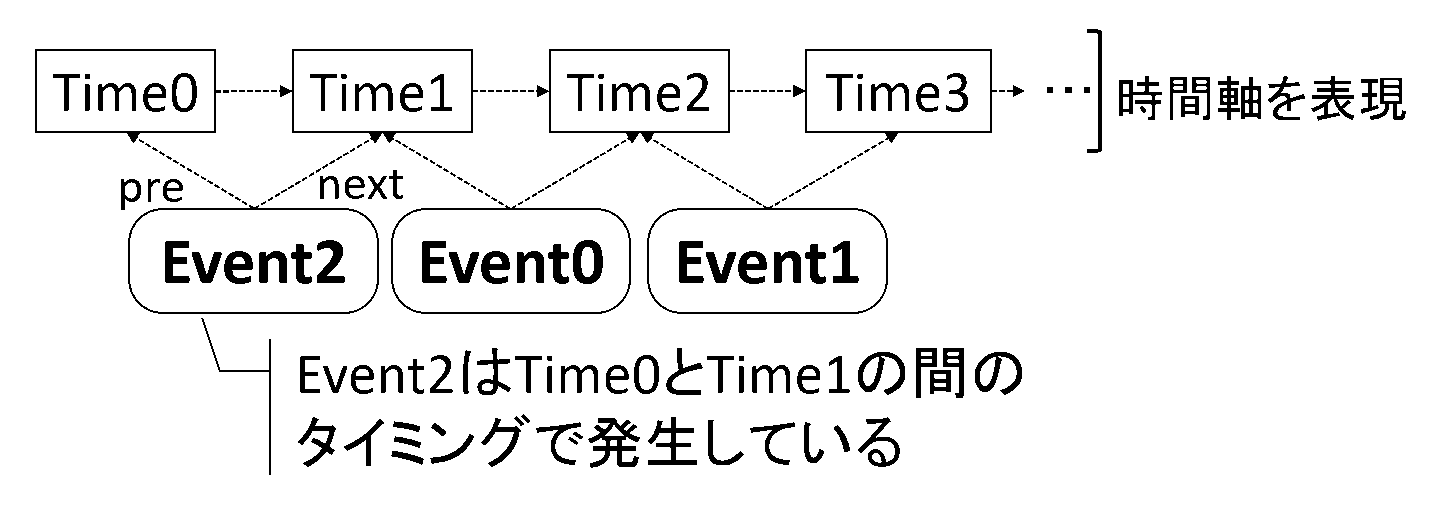
\includegraphics[width=400pt]{./fig/existing-model-temporal-logic.eps}
\caption{基礎モデルにおける時間軸とイベントの対応}
\label{fig:existing-model-temporal-logic}
\end{figure}
\color{black}

\section{Cookieを包括するモデル}
\subsection{モデルの特徴}
Ryckらによって提案されたウェブセキュリティモデル\cite{cookie-model}(以下
、Cookieモデルとする)は、Akhaweらの基礎モデル(\ref{sec:based-model}節参照)を基にCookieの要素を追加したものである。

\subsection{Cookieモデルの能力}
\subsection{Cookieモデルにおける時相論理の実装}

\section{既存モデルにおける不足点}

\end{document}
